% Drawing 146/04-15 -- folder 146, batch 04, archive page 77 (PDF page 78).
% Transcription: Un ruban hexagonal hachuré, replié sur lui-même ; plusieurs graphes trivalents en forme de « nœud papillon » ou de deux triangles joints par une arête, certains avec des sommets cerclés ou hachurés ; une grande ellipse au crayon traversée par un segment ; un réseau en zigzag de quadrilatères et de triangles ; un segment portant trois points ; une boucle à deux points cerclés ; un triangle dont un sommet est cerclé, prolongé par une queue.
% Kind: page of sketches (hexagonal ribbon, trivalent graphs, ellipse, zigzag net). Method 2 (schematic redraw from the facsimile). Status: partial.
% Notes: Drawn over a typed departmental notice (its text, which names a colleague, is not his and is not reproduced). Redrawn by main strokes: the hatched hexagonal ribbon folded on itself (top); the « bow-tie » / two-triangles trivalent graphs (three at the left, one at the right), the pencil ellipse crossed by a segment with a marked point, the zigzag net of quadrilaterals and triangles (lower right) with the segment carrying three points under it, the loop with two ringed points and the triangle with a ringed vertex and a tail. The pencil doublings of each graph (he redrew each two or three times) are reduced to one; which vertices are ringed or hatched is approximate.
% Coordinates: 1 unit = 1 mm = 1/100 of the crop width (bbox in page fractions: [0.13, 0.17, 0.83, 0.85]).
% Redrawn by Claude (claude-opus-5-5), issue #73 pilot, 2026-11-07; not checked by a human; not compiled (no TeX in the session).
% Rights: reproduces part of the work -- behind RENDER_TRANSCRIPTS, never published by itself.
\documentclass[tikz,border=3pt]{standalone}
\usepackage{amsmath,amssymb}
\usetikzlibrary{patterns,arrows.meta}
\tikzset{pencil/.style={black!45}, struck/.style={black!35}, mark/.style={circle,draw,inner sep=1.3pt}, pt/.style={circle,fill,inner sep=0.9pt}, opt/.style={circle,draw,fill=white,inner sep=1.1pt}}
\begin{document}
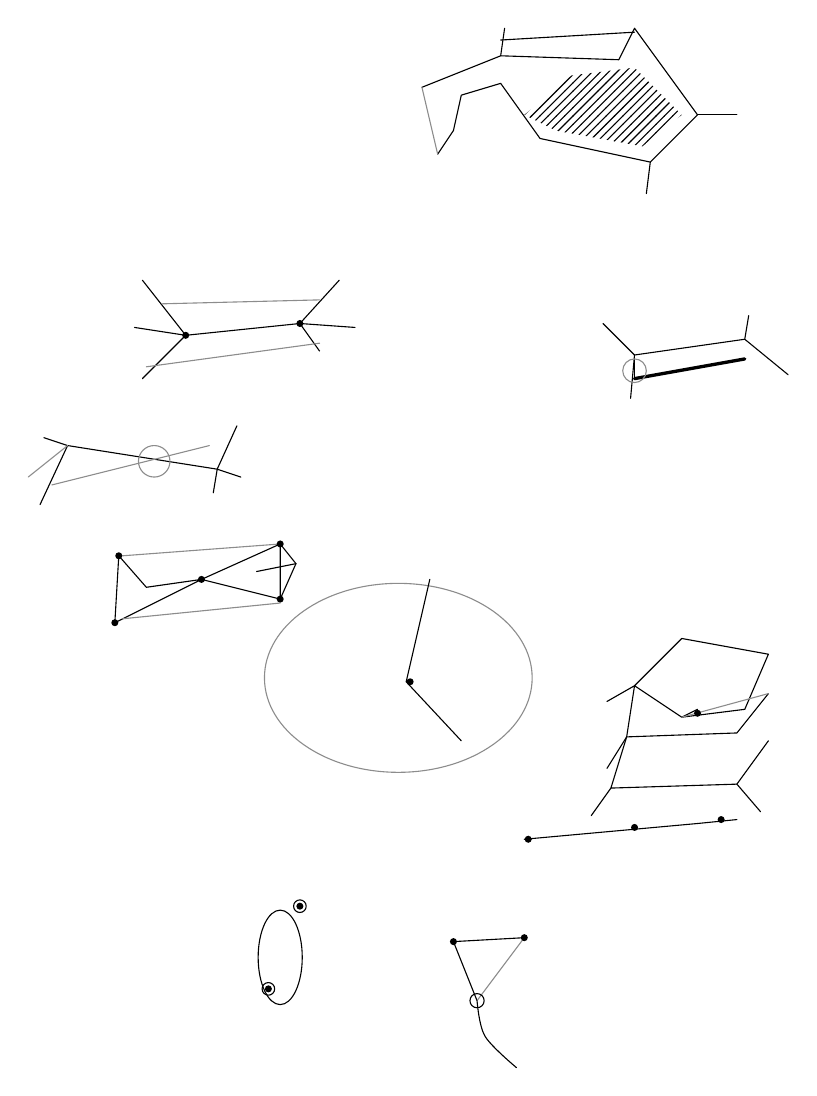
\begin{tikzpicture}[x=1mm,y=1mm,line cap=round,line join=round,font=\scriptsize]
\draw (53,-10.5) -- (63,-6.5) -- (78,-7) -- (80,-3) -- (88,-14) -- (82,-20) -- (68,-17) -- (63,-10) -- (58,-11.5) -- (57,-16);
\draw (63,-6.5) -- (63.5,-3);
\draw (88,-14) -- (93,-14);
\draw (82,-20) -- (81.5,-24);
\draw (55,-19) -- (57,-16);
\draw[pencil] (53,-10.5) -- (55,-19);
\draw plot[smooth, tension=0.55] coordinates {(63,-4.5) (80,-3.5)};
\fill[pattern=north east lines] (66,-14) -- (72,-9) -- (80,-8) -- (86,-14) -- (81,-18) -- (70,-16) -- cycle;
\draw (17.5,-35) -- (23,-42) -- (37.5,-40.5) -- (42.5,-35);
\draw (16.5,-41) -- (23,-42) -- (17.5,-47.5);
\draw (37.5,-40.5) -- (40,-44);
\draw (37.5,-40.5) -- (44.5,-41);
\draw[pencil] (20,-38) -- (40,-37.5);
\draw[pencil] (18,-46) -- (40,-43);
\node[pt] at (23,-42) {};
\node[pt] at (37.5,-40.5) {};
\draw (76,-40.5) -- (80,-44.5) -- (94,-42.5) -- (94.5,-39.5);
\draw (80,-44.5) -- (79.5,-50);
\draw (94,-42.5) -- (99.5,-47);
\draw[very thick] (80,-47.5) -- (94,-45);
\draw (80,-44.5) -- (80,-47.5);
\draw[pencil] (80,-46.5) circle[radius=1.5];
\draw (5,-55) -- (8,-56) -- (27,-59) -- (29.5,-53.5);
\draw (8,-56) -- (4.5,-63.5);
\draw (27,-59) -- (26.5,-62);
\draw (27,-59) -- (30,-60);
\draw[pencil] (3,-60) -- (8,-56);
\draw[pencil] (6,-61) -- (26,-56);
\draw[pencil] (19,-58) circle[radius=2];
\draw (14.5,-70) -- (14,-78.5) -- (25,-73) -- (35,-68.5) -- (35,-75.5) -- (25,-73) -- (18,-74) -- (14.5,-70);
\draw (35,-68.5) -- (37,-71);
\draw (35,-75.5) -- (37,-71);
\draw (32,-72) -- (37,-71);
\draw[pencil] (15,-70) -- (35,-68.5);
\draw[pencil] (15,-78) -- (35,-76);
\node[pt] at (14.5,-70) {};
\node[pt] at (14,-78.5) {};
\node[pt] at (25,-73) {};
\node[pt] at (35,-68.5) {};
\node[pt] at (35,-75.5) {};
\draw[pencil] (50,-85.5) ellipse[x radius=17, y radius=12];
\draw (54,-73) -- (51,-86) -- (58,-93.5);
\node[pt] at (51.5,-86) {};
\draw (80,-86.5) -- (86,-80.5) -- (97,-82.5) -- (94,-89.5) -- (86,-90.5) -- (80,-86.5);
\draw (86,-90.5) -- (88,-89.5);
\draw (80,-86.5) -- (79,-93);
\draw (76.5,-97) -- (79,-93) -- (93,-92.5) -- (97,-87.5);
\draw (79,-93) -- (77,-99.5) -- (93,-99) -- (97,-93.5);
\draw (77,-99.5) -- (74.5,-103);
\draw (93,-99) -- (96,-102.5);
\draw (76.5,-88.5) -- (80,-86.5);
\draw[pencil] (86,-90.5) -- (97,-87.5);
\node[pt] at (88,-90) {};
\draw (66,-106) -- (88,-104) -- (93,-103.5);
\node[pt] at (66.5,-106) {};
\node[pt] at (80,-104.5) {};
\node[pt] at (91,-103.5) {};
\draw (35,-121) ellipse[x radius=2.8, y radius=6];
\draw (37.5,-114.5) circle[radius=0.8];
\draw (33.5,-125) circle[radius=0.8];
\node[pt] at (37.5,-114.5) {};
\node[pt] at (33.5,-125) {};
\draw (57,-119) -- (66,-118.5);
\draw (57,-119) -- (60,-126.5);
\draw[pencil] (66,-118.5) -- (60,-126.5);
\draw plot[smooth, tension=0.55] coordinates {(60,-126.5) (61,-131) (65,-135)};
\node[pt] at (57,-119) {};
\node[pt] at (66,-118.5) {};
\draw (60,-126.5) circle[radius=0.9];
\end{tikzpicture}
\end{document}
